\documentclass[11pt,a4paper]{article}

% IOS Press FAIA style packages
\usepackage[utf8]{inputenc}
\usepackage[T1]{fontenc}
\usepackage{newunicodechar}
\DeclareTextCommandDefault{\h}[1]{#1}
\usepackage{times}
\usepackage{amsmath,amssymb}
\usepackage{graphicx}
\usepackage{booktabs}
\usepackage{multirow}
\usepackage{url}
\usepackage{float}
\usepackage[hidelinks]{hyperref}

% TikZ for diagrams
\usepackage{tikz}
\usetikzlibrary{shapes.geometric, arrows.meta, positioning, fit, backgrounds, calc}

% pgfplots for charts
\usepackage{pgfplots}
\pgfplotsset{compat=1.18}

% checkmark
\usepackage{amssymb}

% Page layout for IOS Press
\usepackage[top=2.3cm,bottom=2.3cm,left=2cm,right=2cm]{geometry}
\setlength{\parindent}{0.5cm}
\setlength{\parskip}{0pt}

% Two-column layout
\usepackage{multicol}
\setlength{\columnsep}{0.5cm}

% Section formatting
\usepackage{titlesec}
\titleformat{\section}{\normalfont\bfseries}{\thesection.}{0.5em}{}
\titleformat{\subsection}{\normalfont\bfseries\itshape}{\thesubsection.}{0.5em}{}
\titleformat{\subsubsection}{\normalfont\itshape}{\thesubsubsection.}{0.5em}{}
\titlespacing*{\section}{0pt}{1.2ex plus 0.5ex minus 0.2ex}{0.8ex plus 0.2ex}
\titlespacing*{\subsection}{0pt}{1.0ex plus 0.3ex minus 0.2ex}{0.5ex plus 0.1ex}
\titlespacing*{\subsubsection}{0pt}{0.8ex plus 0.2ex minus 0.1ex}{0.3ex plus 0.1ex}

% Caption formatting
\usepackage{caption}
\captionsetup{font=small,labelfont=bf,skip=4pt}

% Tighter spacing
\setlength{\textfloatsep}{8pt}
\setlength{\floatsep}{6pt}
\setlength{\intextsep}{6pt}

% Ensure text returns to justified after captionof
\usepackage{ragged2e}

\begin{document}

% Title
\begin{center}
{\Large\bfseries A Three-Tier Ontology-Enhanced Retrieval Augmented Generation\\[0.3em] for Vietnamese Legal Question Answering}\\[1.5em]

{\normalsize
Le Hong Hien$^{a,1}$, Nguyen Dinh Hien$^{a}$, Ngo Quoc Hung$^{b}$ and Dang Viet Dung$^{a}$\\[0.5em]
$^a$\textit{Faculty of Computer Science, University of Information Technology,}\\
\textit{Vietnam National University Ho Chi Minh City, Vietnam}\\
$^b$\textit{School of Computer Science, University College Dublin, Ireland}\\[1em]
}
\end{center}

\noindent\textbf{Abstract.} Legal question answering (QA) systems face unique challenges due to complex hierarchical structures, cross-references between articles, and multi-hop reasoning requirements inherent in legal documents. Traditional Retrieval Augmented Generation (RAG) systems rely on vector similarity, which often fails to capture semantic relationships in legal texts. This paper proposes a Three-Tier Ontology-Enhanced RAG architecture that addresses these limitations through: (1) LLM-guided tree traversal for hierarchical document navigation, (2) dual-level semantic retrieval with Multi-Intent Personalized PageRank for graph-based reasoning, and (3) Reciprocal Rank Fusion for cross-tier result merging with knowledge graph expansion. We evaluate our approach on Vietnam Enterprise Law 2020 and related decrees, demonstrating substantial improvements over baseline methods. Our experimental results on 375 real legal questions show that the proposed three-tier method achieves 75.2\% Hit@10, significantly outperforming traditional BM25 (26.7\%), TF-IDF (28.8\%), semantic search (15.8\%), LightRAG (33.9\%), and single-tier PageIndex (35.2\%). Ablation studies confirm that each tier contributes meaningfully, with Tier~3 fusion providing an additional 4.0 percentage point improvement over Tier~1+2 alone. These results demonstrate the effectiveness of combining structural, semantic, and graph-based retrieval for legal domain applications.\\[0.5em]

\noindent\textbf{Keywords.} Ontology, Legal Question Answering, Retrieval Augmented Generation, Knowledge Graph, Vietnamese NLP, Multi-Tier Retrieval

\begin{multicols}{2}

\section{Introduction}

Legal question answering (QA) systems have become increasingly important as citizens and businesses seek to understand their rights and obligations under the law. However, building effective legal QA systems presents unique challenges that distinguish this domain from general-purpose question answering.

First, legal documents contain \textbf{complex hierarchical structures}. A single law may be organized into parts, chapters, sections, articles, clauses, and points, with each level carrying different legal weight and scope. Understanding the relationship between these structural elements is crucial for accurate retrieval.

Second, legal texts frequently contain \textbf{cross-references between articles}. An article defining shareholder rights may reference another article specifying conditions, which in turn references procedures defined elsewhere. Answering a practical question often requires following these reference chains across multiple articles.

Third, legal questions often require \textbf{multi-hop reasoning}. A question like ``Can a foreign investor establish a limited liability company in Vietnam?'' requires understanding: (1) who qualifies as a foreign investor, (2) what types of companies can be established, (3) specific conditions for foreign investment, and (4) procedures for company registration.

Traditional Retrieval Augmented Generation (RAG) \cite{ref2} systems rely primarily on vector similarity between query embeddings and document embeddings \cite{ref_sbert}. While effective for many domains \cite{ref_gao2024,ref_fan2024}, this approach has significant limitations for legal QA:

\begin{itemize}
\item \textbf{Semantic gap}: Legal terminology often has precise meanings that differ from common usage. Vector embeddings trained on general corpora may not capture these domain-specific semantics.
\item \textbf{Missing structural awareness}: Vector similarity treats documents as flat text, ignoring the hierarchical structure that carries legal significance.
\item \textbf{No reasoning capability}: Dense retrieval cannot follow logical chains of references or apply legal inference rules.
\end{itemize}

This paper proposes a \textbf{Three-Tier Ontology-Enhanced RAG} architecture that addresses these limitations. Our approach combines LLM-guided structural navigation with ontology-based semantic retrieval and cross-tier fusion, enabling:

\begin{enumerate}
\item LLM-guided tree traversal through document hierarchies (Tier~1)
\item Dual-level semantic retrieval with intent-aware Personalized PageRank on a domain-specific knowledge graph (Tier~2)
\item Reciprocal Rank Fusion for cross-tier merging with knowledge graph expansion (Tier~3)
\end{enumerate}

We evaluate our approach on Vietnam Enterprise Law 2020 (Law No. 59/2020/QH14) and related decrees, consisting of 10 chapters and 218 articles in the primary law. Our evaluation dataset comprises 375 real legal questions collected from Vietnamese legal consultation platforms, with expert-annotated ground truth relevant articles.

The main contributions of this paper are:

\begin{itemize}
\item \textbf{Three-Tier RAG Architecture}: We propose a novel multi-tier retrieval system combining LLM-guided tree traversal (Tier~1), dual-level semantic retrieval with knowledge graph reasoning (Tier~2), and Reciprocal Rank Fusion with KG expansion (Tier~3).

\item \textbf{Vietnamese Legal Knowledge Graph}: We construct a knowledge graph with 1,299 entities across 11 types and 2,577 relations across 22 types, extracted via LLM-based unified extraction with incremental deduplication.

\item \textbf{Multi-Intent Personalized PageRank}: We propose an intent-aware graph traversal algorithm based on PageRank \cite{ref12} that detects multiple query intents (e.g., penalty, procedure, definition) and adapts edge weights accordingly during propagation.

\item \textbf{Comprehensive Evaluation}: We conduct extensive experiments on 375 real legal questions comparing against multiple baselines including BM25, TF-IDF, Semantic Search, LightRAG \cite{ref5}, and PageIndex, with ablation studies isolating each tier's contribution.
\end{itemize}

The rest of this paper is organized as follows. Section~\ref{sec:related} reviews related work. Section~\ref{sec:background} introduces preliminary concepts. Section~\ref{sec:architecture} describes our three-tier architecture including knowledge graph construction. Section~\ref{sec:experiments} presents experimental results and analysis. Section~\ref{sec:discussion} discusses findings and limitations. Section~\ref{sec:conclusion} concludes the paper.

\section{Related Work}
\label{sec:related}

\subsection{Legal Information Retrieval}

Legal information retrieval has been studied extensively over the past decades. Traditional approaches rely on lexical matching methods such as BM25 and TF-IDF \cite{ref11}. While these methods are efficient and interpretable, they struggle with vocabulary mismatch between user queries and legal terminology.

Recent advances in neural retrieval have introduced dense passage retrieval using transformer-based embeddings \cite{ref3}, building on the Transformer architecture \cite{ref_vaswani}. Retrieval-Augmented Generation (RAG) \cite{ref2} combines retrieval with generation for knowledge-intensive tasks. Comprehensive surveys \cite{ref_gao2024,ref_fan2024} document the rapid progress in RAG systems. Systems like DPR and ColBERT demonstrate strong performance on general QA benchmarks, while domain-specific models such as LEGAL-BERT \cite{ref_chalkidis} adapt pre-trained representations for legal text. However, applying these methods to legal domain requires careful adaptation due to the specialized nature of legal language \cite{ref_zhong2020,ref_legalai2024}.

For Vietnamese legal text processing, pre-trained models such as PhoBERT \cite{ref_phobert} and tools like VnCoreNLP \cite{ref_vncorenlp} have advanced Vietnamese NLP capabilities. Ngo et al. \cite{ref7} designed a legal QA system leveraging BM25, pre-trained BERT \cite{ref13} models, and legal domain knowledge. They proposed data augmentation based on legal domain knowledge for textual entailment. However, their approach does not explicitly represent the semantic structure of legal documents.

\subsection{Knowledge Graphs for Legal Domain}

Ontology-based approaches have shown promise for representing legal knowledge \cite{ref8}. Knowledge graph embedding methods such as TransE \cite{ref_transe} and RotatE \cite{ref_rotateE} provide foundational techniques for learning entity representations in multi-relational graphs. LIDO (Legal Informatics Document Ontology) provides a framework for representing legal actions, temporal events, and document structure. The CEN Metalex standard defines XML interchange formats for legal resources.

Legal-Onto \cite{ref6} proposed an integration of ontology Rela-model \cite{ref10} with conceptual graphs for Vietnamese Land Law. This approach represents concepts, relations, and inference rules specific to the legal domain. Our work extends this foundation by integrating ontology-based retrieval with modern RAG systems for question answering.

\subsection{Graph-based RAG Systems}

Recent work has explored graph-augmented retrieval for knowledge-intensive tasks. Microsoft's GraphRAG \cite{ref4} uses knowledge graphs constructed from documents to enable global summarization and multi-hop reasoning. LightRAG \cite{ref5} provides a lightweight alternative focusing on entity extraction and relationship modeling.

Other RAG variants address retrieval quality from different angles: Self-RAG \cite{ref_selfrag} adds self-reflection to filter irrelevant passages, CRAG \cite{ref_crag} incorporates corrective retrieval mechanisms, and HyDE \cite{ref_hyde} generates hypothetical documents to improve retrieval. However, these general-purpose graph RAG systems construct knowledge graphs automatically without domain expertise. For legal domain, the precision of concept extraction and relationship modeling is crucial \cite{ref_wadhwa}.

PageIndex \cite{ref14} introduced LLM-guided tree traversal for hierarchical document navigation, using document structure summaries to guide retrieval. Our work combines this structural navigation approach with ontology-based semantic retrieval and cross-tier fusion, creating a multi-tier system that leverages both document hierarchy and knowledge graph reasoning.

Table~\ref{tab:related-comparison} summarizes the key features of related systems compared to our approach.

\vspace{0.3em}
\noindent
\centering\scriptsize
\captionof{table}{Feature Comparison of RAG Systems}
\label{tab:related-comparison}
\begin{tabular}{l@{\hskip 4pt}c@{\hskip 4pt}c@{\hskip 4pt}c@{\hskip 4pt}c@{\hskip 4pt}c}
\toprule
\textbf{Feature} & \textbf{BM25} & \textbf{Light} & \textbf{Graph} & \textbf{Page} & \textbf{Ours} \\
\midrule
Knowledge Graph & -- & \checkmark & \checkmark & -- & \checkmark \\
Multi-tier & -- & -- & -- & -- & \checkmark \\
Intent-aware & -- & -- & -- & -- & \checkmark \\
Domain Ontology & -- & -- & -- & -- & \checkmark \\
Tree Navigation & -- & -- & -- & \checkmark & \checkmark \\
Rank Fusion & -- & -- & -- & -- & \checkmark \\
\bottomrule
\end{tabular}
\normalsize
\justifying
\vspace{0.3em}

\section{Preliminaries}
\label{sec:background}

\textbf{Personalized PageRank (PPR)} \cite{ref12,ref_jeh2003} computes query-specific node importance on a graph. The PPR vector $\pi$ satisfies $\pi = (1-\alpha) \cdot \tilde{A}^T \pi + \alpha \cdot p$, where $\tilde{A}$ is the column-normalized adjacency matrix, $\alpha$ is the teleport probability, and $p$ is the personalization vector seeded from matched entities.

\textbf{Reciprocal Rank Fusion (RRF)} \cite{ref_rrf} aggregates multiple ranked lists: $\text{RRF}(d) = \sum_{r \in \mathcal{R}} \frac{1}{k + \text{rank}_r(d)}$, where $k=60$ is a smoothing constant. RRF handles heterogeneous score distributions without normalization, making it suitable for combining LLM-based discrete selections with continuous semantic scores.

\textbf{Legal Document Ontology.} Our ontology extends the Rela-model \cite{ref10} for Vietnamese legal knowledge. Documents are modeled as hierarchical trees (Document $\rightarrow$ Chapter $\rightarrow$ Article $\rightarrow$ Clause $\rightarrow$ Point) with typed entities and semantic relations extracted from article text.

\section{System Architecture}
\label{sec:architecture}

Our system consists of two main phases: offline knowledge graph construction and online three-tier query processing. Figure~\ref{fig:architecture} illustrates the overall architecture.

\end{multicols}

% Figure 1: System Architecture
\begin{figure}[H]
\centering
\resizebox{\textwidth}{!}{%
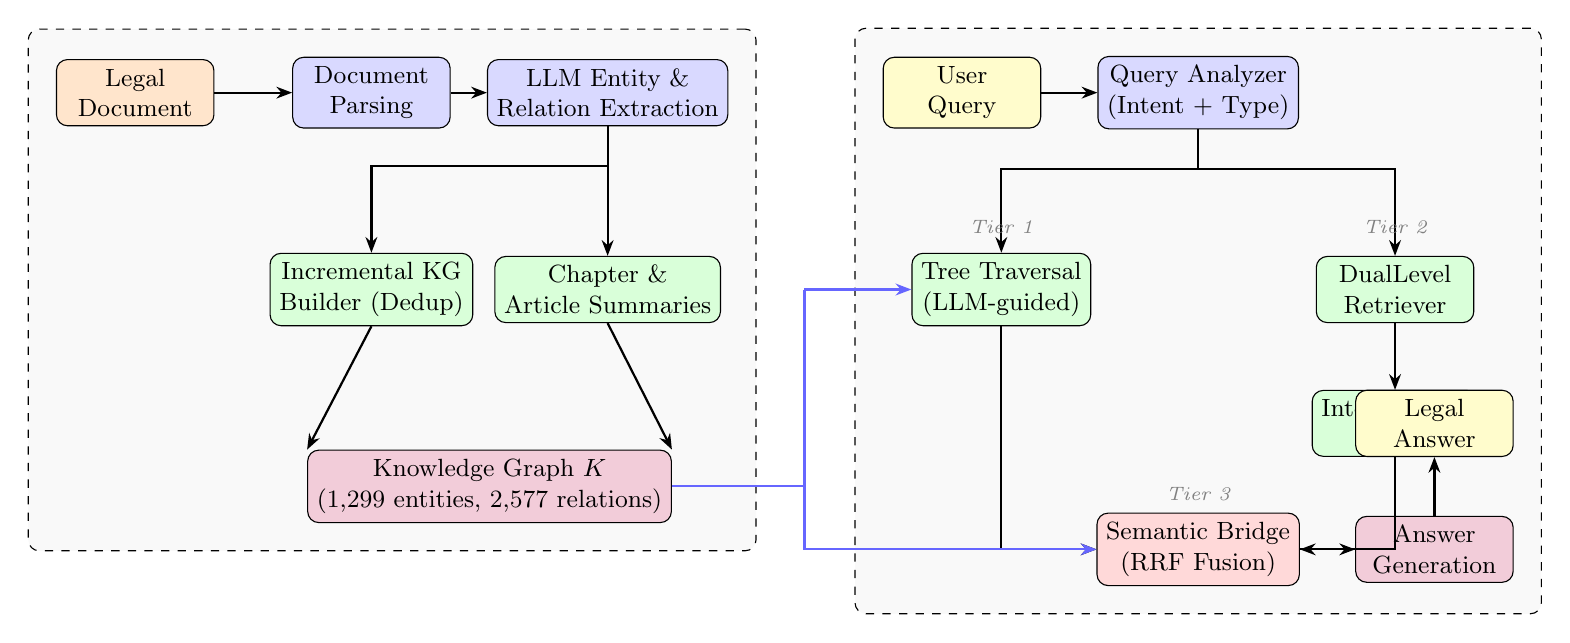
\begin{tikzpicture}[
    % Styles
    box/.style={rectangle, draw, rounded corners, minimum height=0.8cm, minimum width=2cm, align=center, font=\small},
    phase/.style={rectangle, draw, dashed, rounded corners, inner sep=10pt},
    tier/.style={rectangle, draw, dashed, rounded corners, inner sep=8pt, fill=blue!3},
    arrow/.style={-{Stealth[length=2mm]}, thick},
    dataarrow/.style={-{Stealth[length=2mm]}, thick, blue!60},
    label/.style={font=\footnotesize\bfseries},
]

% === OFFLINE PHASE (Left) ===
\node[box, fill=orange!20] (doc) at (0,0) {Legal\\Document};
\node[box, fill=blue!15] (parse) at (3,0) {Document\\Parsing};
\node[box, fill=blue!15] (extract) at (6,0) {LLM Entity \&\\Relation Extraction};
\node[box, fill=green!15] (kgbuild) at (3,-2.5) {Incremental KG\\Builder (Dedup)};
\node[box, fill=green!15] (summary) at (6,-2.5) {Chapter \&\\Article Summaries};
\node[box, fill=purple!20, minimum width=3cm] (kg) at (4.5,-5) {Knowledge Graph $K$\\(1,299 entities, 2,577 relations)};

% Offline arrows
\draw[arrow] (doc) -- (parse);
\draw[arrow] (parse) -- (extract);
\draw[arrow] (extract.south) -- ++(0,-0.5) -| (kgbuild.north);
\draw[arrow] (extract.south) -- ++(0,-0.5) -| (summary.north);
\draw[arrow] (kgbuild.south) -- (kg.north west);
\draw[arrow] (summary.south) -- (kg.north east);

% Offline phase box
\begin{scope}[on background layer]
\node[phase, fill=gray!5, fit=(doc)(parse)(extract)(kgbuild)(summary)(kg), label={[label]above:Offline Phase: KG Construction}] (offline) {};
\end{scope}

% === ONLINE PHASE (Right) ===
\node[box, fill=yellow!20] (query) at (10.5,0) {User\\Query};
\node[box, fill=blue!15] (analyzer) at (13.5,0) {Query Analyzer\\(Intent + Type)};

% Tier 1
\node[box, fill=green!15] (tree) at (11,-2.5) {Tree Traversal\\(LLM-guided)};

% Tier 2
\node[box, fill=green!15] (dual) at (16,-2.5) {DualLevel\\Retriever};
\node[box, fill=green!15] (ppr) at (16,-4.2) {Intent-Aware\\PPR};

% Tier 3
\node[box, fill=red!15] (bridge) at (13.5,-5.8) {Semantic Bridge\\(RRF Fusion)};
\node[box, fill=purple!20] (gen) at (16.5,-5.8) {Answer\\Generation};
\node[box, fill=yellow!20] (answer) at (16.5,-4.2) {Legal\\Answer};

% Online arrows
\draw[arrow] (query) -- (analyzer);
\draw[arrow] (analyzer.south) -- ++(0,-0.5) -| (tree.north);
\draw[arrow] (analyzer.south) -- ++(0,-0.5) -| (dual.north);
\draw[arrow] (dual) -- (ppr);
\draw[arrow] (tree.south) |- (bridge.west);
\draw[arrow] (ppr.south) |- (bridge.east);
\draw[arrow] (bridge) -- (gen);
\draw[arrow] (gen) -- (answer);

% KG to Online connections
\coordinate (splitpt) at (8.5,-5);
\draw[blue!60, thick] (kg.east) -- (splitpt);
\draw[blue!60, thick] (splitpt) -- (8.5,-2.5);
\draw[dataarrow] (8.5,-2.5) -- (tree.west);
\draw[dataarrow] (splitpt) -- (8.5,-5.8) -- (bridge.west);

% Tier labels
\node[font=\scriptsize\itshape, gray] at (11,-1.7) {Tier 1};
\node[font=\scriptsize\itshape, gray] at (16,-1.7) {Tier 2};
\node[font=\scriptsize\itshape, gray] at (13.5,-5.1) {Tier 3};

% Online phase box
\begin{scope}[on background layer]
\node[phase, fill=gray!5, fit=(query)(analyzer)(tree)(dual)(ppr)(bridge)(gen)(answer), label={[label]above:Online Phase: Three-Tier Query Processing}] (online) {};
\end{scope}

\end{tikzpicture}
}
\caption{System architecture overview. The offline phase constructs knowledge graph $K$ from legal documents. The online phase processes queries through three tiers: LLM-guided tree traversal (Tier~1), dual-level semantic retrieval with PPR (Tier~2), and RRF-based fusion (Tier~3).}
\label{fig:architecture}
\end{figure}

\begin{multicols}{2}

\subsection{Knowledge Representation}

Our knowledge representation builds upon the Legal-Onto framework \cite{ref6}, which integrates the Rela-model \cite{ref10} with conceptual graphs for legal knowledge. We extend this with a hierarchical document model:

\begin{equation}
K = (E, R, T) + (Forest, Summaries)
\end{equation}

where:
\begin{itemize}
\item $E$: A set of legal entities with typed attributes (11 entity types)
\item $R$: A set of typed relations between entities (22 relation types)
\item $T$: A document tree forest (Document $\rightarrow$ Chapter $\rightarrow$ Article $\rightarrow$ Clause $\rightarrow$ Point)
\item $Forest$: A collection of hierarchical document trees for structural navigation
\item $Summaries$: LLM-generated chapter and article summaries for tree traversal
\end{itemize}

Each entity $e \in E$ is a tuple:
\begin{equation}
e = (id, name, type, src, meta, conf)
\end{equation}
where $id$ is a Vietnamese slug (e.g., \textit{cong-ty-co-phan}), $type \in$ \{11 legal entity types\}, $src$ links to source articles, and $conf$ tracks extraction confidence.

Entity types include: Organization, Person/Role, Legal Term, Legal Reference, Monetary, Percentage, Duration, Condition, Action, and Penalty. Relation types include: \textit{requires}, \textit{has\_authority}, \textit{permits}, \textit{includes}, \textit{defines\_as}, \textit{references}, \textit{applies\_to}, and others.

This dual representation---knowledge graph for semantic reasoning and document forest for structural navigation---enables our three-tier retrieval approach. The \textbf{Offline Phase} constructs $K$ through LLM-based extraction, while the \textbf{Online Phase} leverages $K$ across three parallel retrieval tiers.

\subsection{Offline Phase: Knowledge Graph Construction}

The offline phase builds the legal knowledge graph and document forest through a semi-automated pipeline:

\textbf{Step 1: Document Parsing.} We parse legal documents according to their hierarchical structure (Chapter $\rightarrow$ Section $\rightarrow$ Article $\rightarrow$ Clause $\rightarrow$ Point). Each structural element is stored in a SQLite database with SQLAlchemy ORM, preserving position, parent-child relationships, cross-references, and full text content. The resulting document tree forms the \textit{UnifiedForest} data structure used by Tier~1 retrieval.

\textbf{Step 2: Unified Entity-Relation Extraction.} We employ a single LLM call per article (using Gemini/GPT-4o-mini) to extract both entities and relations simultaneously, inspired by LightRAG \cite{ref5}. The prompt instructs the model to identify 11 entity types (Organization, Role, Legal Term, Reference, Monetary, Percentage, Duration, Condition, Action, Penalty, Location) and produce evidence-grounded relations between them.

\textbf{Step 3: Incremental KG Building.} Extracted entities are deduplicated in real-time using Vietnamese slug normalization (Unicode NFD, diacritics removal, e.g., ``C\^ong ty c\h{o} ph\`an'' $\rightarrow$ \textit{cong-ty-co-phan}). This LightRAG-inspired in-place merging strategy maintains $O$(unique entities) memory complexity rather than accumulating all extractions before deduplication. Entity confidence is tracked across multiple occurrences.

\textbf{Step 4: Summary Generation.} LLM-generated summaries are produced for each chapter and article, enabling the tree traversal retriever (Tier~1) to make informed navigation decisions without reading full article text during search.

\textbf{Step 5: Abbreviation Dictionary.} A domain-specific dictionary of 50+ Vietnamese legal abbreviations is maintained (e.g., \textit{H\DJ QT} $\rightarrow$ \textit{H\d{o}i d\`{o}ng qu\h{a}n tr\d{i}}, \textit{CTCP} $\rightarrow$ \textit{C\^{o}ng ty c\h{o} ph\`{a}n}), supporting query expansion at search time.

\subsection{Online Phase: Three-Tier Query Processing}

When a user submits a question, the system processes it through query analysis followed by three parallel retrieval tiers.

\textbf{Stage 0: Query Analysis.} The \textit{VietnameseLegalQueryAnalyzer} performs multi-faceted query understanding:
\begin{itemize}
\item \textbf{Intent detection} (6 types): Penalty, Definition, Procedure, Requirement, Reference, General---using Vietnamese regex patterns with LLM fallback
\item \textbf{Query type classification} (7 types): Article lookup, Guidance document, Situation analysis, Compare regulations, Case law lookup, Timeline history, General---each mapped to retrieval strategy parameters
\item \textbf{Abbreviation expansion}: Vietnamese legal abbreviations are expanded (e.g., \textit{TNHH} $\rightarrow$ \textit{tr\'ach nhi\d{e}m h\~{u}u h\d{a}n})
\item \textbf{Ontology expansion}: Query terms are expanded via class hierarchy (children, parents, siblings)
\end{itemize}

\subsubsection{Tier 1: LLM-Guided Tree Traversal}

Inspired by PageIndex, Tier~1 navigates the document hierarchy using LLM reasoning in three loops:

\begin{enumerate}
\item \textbf{Loop 0 (Forest $\rightarrow$ Document)}: LLM selects top 3 relevant documents from summaries
\item \textbf{Loop 1 (Document $\rightarrow$ Chapter)}: LLM selects top 6 relevant chapters using chapter summaries and detected keywords
\item \textbf{Loop 2 (Chapter $\rightarrow$ Article)}: LLM identifies top 7 specific articles from article summaries within selected chapters
\end{enumerate}

General Provisions chapters are automatically included when specific chapters are selected. Each loop produces a reasoning path enabling interpretable retrieval.

\subsubsection{Tier 2: Dual-Level Semantic Retrieval}

Tier~2 performs hybrid semantic search with six scoring components:

\textbf{Low-level (entity-specific):}
\begin{itemize}
\item \textbf{Keyphrase matching}: Query keyphrases matched against article text
\item \textbf{Semantic search}: Cosine similarity between query and entity embeddings
\item \textbf{PPR scoring}: Intent-aware Personalized PageRank on knowledge graph
\item \textbf{Concept matching}: Ontology class matching via expansion
\end{itemize}

\textbf{High-level (theme/concept):}
\begin{itemize}
\item \textbf{Theme matching}: Legal theme identification (penalties, rights, procedures)
\item \textbf{Hierarchy traversal}: Upward/downward ontology class navigation
\end{itemize}

The final Tier~2 score fuses all six components:
\begin{multline}
S_{\text{T2}} = 0.05 S_{\text{kp}} + 0.20 S_{\text{con}} + 0.25 S_{\text{PPR}} \\
+ 0.20 S_{\text{sem}} + 0.15 S_{\text{thm}} + 0.15 S_{\text{hier}}
\end{multline}

\textbf{Multi-Intent Personalized PageRank.} The PPR component uses intent-aware edge weights. The score for node $v$ is:
\begin{equation}
\text{PPR}(v) = (1-\alpha) \sum_{u \in N(v)} \frac{w(u,v) \cdot \text{PPR}(u)}{d(u)} + \alpha \cdot p(v)
\end{equation}
where $\alpha=0.15$ is the teleport probability, $w(u,v)$ is the edge weight adjusted by query intent, $d(u)$ is the out-degree of $u$, and $p(v)$ is the personalization vector seeded from matched entities. Different relation types receive different weights based on detected intent (e.g., \textit{has\_authority} weighted 1.0 for right-related queries vs 0.5 for procedure queries).

\subsubsection{Tier 3: Semantic Bridge (RRF Fusion)}

Tier~3 merges results from Tier~1 and Tier~2 using Reciprocal Rank Fusion (RRF):
\begin{equation}
\text{RRF}(d) = \sum_{s \in \{T1, T2, KG\}} w_s \cdot \frac{1}{k + \text{rank}_s(d)}
\end{equation}
where $k=60$ is the standard RRF constant and source weights are $w_{T1}=0.8$ (tree), $w_{T2}=1.0$ (dual-level), $w_{KG}=1.2$ (KG expansion). RRF is particularly suited here because it is rank-agnostic, handling the different score scales from LLM-based tree selection and continuous semantic scores.

\textbf{Adjacent article expansion.} After RRF scoring, we expand $\pm 2$ articles from each selected article with a decay factor of 0.7. Error analysis showed that failures often have the correct answer within $\pm 3$ articles of a retrieved result, making this expansion effective for recall improvement.

\textbf{Answer Generation.} Top-ranked articles are passed to an LLM for answer generation with citation instructions.

\subsection{Knowledge Graph Details}

Our constructed knowledge graph for Vietnam Enterprise Law 2020 and related decrees is summarized in Table~\ref{tab:kg-stats}. Each entity is stored as a merged record with Vietnamese slug ID, typed attributes, source article links, aliases, and confidence scores. Relations are keyed by \texttt{source\_slug|predicate|target\_slug} with evidence text for interpretable traversal.

\end{multicols}

\begin{table}[H]
\centering\small
\caption{Knowledge Graph Statistics}
\label{tab:kg-stats}
\begin{tabular}{lr@{\hskip 2cm}lr@{\hskip 2cm}lr}
\toprule
\textbf{Entity Type} & \textbf{Count} & \textbf{Relation Type} & \textbf{Count} & \textbf{Structure} & \textbf{Count} \\
\midrule
Total Entities & 1,299 & Total Relations & 2,577 & Document Tree Nodes & 1,847 \\
Organization & 187 & requires & 423 & Chapter Summaries & 10 \\
Person/Role & 156 & has\_authority & 312 & Article Summaries & 218 \\
Legal Term & 234 & applies\_to & 287 & & \\
Legal Reference & 198 & references & 265 & & \\
Condition & 178 & includes & 234 & & \\
Action & 163 & defines\_as & 198 & & \\
Other types & 183 & Other relations & 858 & & \\
\bottomrule
\end{tabular}
\end{table}

\begin{multicols}{2}

\subsubsection{Intent-Aware Edge Weights}

Different query intents prioritize different relation types. We define intent-specific weight multipliers for the PPR algorithm:

\vspace{0.3em}
\noindent
\centering\small
\captionof{table}{Intent-Relation Weight Matrix}
\label{tab:intent-weights}
\begin{tabular}{l@{\hskip 4pt}c@{\hskip 4pt}c@{\hskip 4pt}c@{\hskip 4pt}c@{\hskip 4pt}c}
\toprule
\textbf{Relation} & \textbf{Def.} & \textbf{Proc.} & \textbf{Right} & \textbf{Obl.} & \textbf{Pen.} \\
\midrule
defines\_as & 1.0 & 0.5 & 0.5 & 0.5 & 0.5 \\
includes & 0.95 & 0.5 & 0.5 & 0.5 & 0.5 \\
requires & 0.5 & 1.0 & 0.5 & 0.85 & 0.5 \\
has\_authority & 0.5 & 0.5 & 1.0 & 0.5 & 0.5 \\
has\_obligation & 0.5 & 0.5 & 0.5 & 1.0 & 0.5 \\
has\_penalty & 0.5 & 0.5 & 0.5 & 0.5 & 1.0 \\
\bottomrule
\end{tabular}
\normalsize
\justifying
\vspace{0.3em}

For definition queries, \textit{defines\_as} and \textit{includes} edges receive higher weight (1.0, 0.95). For procedure queries, \textit{requires} is prioritized. This allows the PPR algorithm to traverse the graph along paths most relevant to the query intent, improving retrieval precision for intent-specific questions.

\section{Experiments}
\label{sec:experiments}

\subsection{Dataset}

We evaluate on Vietnam Enterprise Law 2020 and related decrees with the following characteristics:

\begin{itemize}
\item \textbf{Legal corpus}: 10 chapters, 218 articles in the primary Enterprise Law (No. 59/2020/QH14), plus 9 related decrees covering implementation details
\item \textbf{Evaluation questions}: 375 real questions collected from Vietnamese legal consultation platforms (LuatVietnam, ThuVienPhapLuat, legal forums)
\item \textbf{Ground truth}: Expert-annotated relevant articles by legal professionals. Each question has 1--8 relevant articles (average: 2.3)
\item \textbf{Question categories}: Article lookup (41.6\%), Guidance document (26.1\%), Situation analysis (20.0\%), Compare regulations (8.5\%), Case law lookup (3.8\%)
\end{itemize}

\subsection{Baselines}

We compare against five baseline methods:

\textbf{BM25} \cite{ref1}: Traditional lexical retrieval using Okapi BM25 scoring with Vietnamese tokenization. Parameters: $k_1=1.2$, $b=0.75$.

\textbf{TF-IDF} \cite{ref11}: Term frequency--inverse document frequency with Vietnamese word segmentation and cosine similarity ranking.

\textbf{Semantic Search} \cite{ref_sbert}: Dense retrieval using sentence-transformers (\texttt{paraphrase-multilingual-\allowbreak{}MiniLM-L12-v2}) embeddings. We embed each article and retrieve by cosine similarity.

\textbf{LightRAG} \cite{ref5}: Graph-based RAG using automatic entity extraction and relationship modeling. We use the official implementation with default parameters.

\textbf{PageIndex}: Tree traversal only (our Tier~1 in isolation), representing structured LLM-guided retrieval without semantic search or KG reasoning.

\subsection{Evaluation Metrics}

\textbf{Retrieval Metrics} (computed at $k \in \{1,3,5,10,20,30,50\}$):
\begin{itemize}
\item \textbf{Hit@k}: Whether at least one relevant article appears in top $k$ results
\item \textbf{Recall@k}: Proportion of relevant articles retrieved in top $k$
\item \textbf{NDCG@k}: Normalized Discounted Cumulative Gain
\item \textbf{MRR}: Mean Reciprocal Rank of the first relevant result
\end{itemize}

\subsection{Implementation Details}

We use Claude 3.5 Haiku for tree traversal/query analysis and Gemini 2.0 Flash for entity extraction. Embeddings are from sentence-transformers (\texttt{paraphrase-multilingual-\allowbreak{}MiniLM-L12-v2}) \cite{ref_sbert}. The KG uses iterative PPR (max 50 iterations, tolerance $10^{-6}$). All LLM responses are cached in SQLite ($\sim$1.1\,GB) for reproducibility.

\subsection{Results}

\subsubsection{Retrieval Performance}

Table~\ref{tab:main-results} presents Hit@k retrieval performance comparison across all methods.

\vspace{0.3em}
\noindent
\centering\small
\captionof{table}{Hit@k Performance (\%). Best \textbf{bold}, 2nd \underline{underlined}.}
\label{tab:main-results}
\begin{tabular}{l@{\hskip 3pt}r@{\hskip 3pt}r@{\hskip 3pt}r@{\hskip 3pt}r@{\hskip 3pt}r@{\hskip 3pt}r}
\toprule
\textbf{Method} & \textbf{@5} & \textbf{@10} & \textbf{@20} & \textbf{@30} & \textbf{@50} & \textbf{Avg. Art.} \\
\midrule
Semantic & 7.4 & 15.8 & 38.5 & 44.3 & 48.3 & 50.0 \\
BM25 & 15.0 & 26.7 & 50.1 & 58.1 & 79.2 & 50.0 \\
TF-IDF & 15.8 & 28.8 & 50.7 & 62.0 & \underline{82.3} & 50.0 \\
LightRAG & 18.8 & 33.9 & \underline{51.0} & \underline{66.2} & 70.3 & 32.8 \\
PageIndex & \underline{31.7} & \underline{35.2} & 35.2 & 35.2 & 35.2 & 3.9 \\
\textbf{3-Tier (ours)} & \textbf{68.5} & \textbf{75.2} & \textbf{82.1} & \textbf{84.0} & \textbf{86.4} & 52.3 \\
\bottomrule
\end{tabular}
\normalsize
\justifying
\vspace{0.3em}
\justifying

Key observations:
\begin{itemize}
\item \textbf{Semantic search performs poorly} (15.8\% Hit@10) due to general-purpose embeddings failing to capture Vietnamese legal semantics.
\item \textbf{BM25 and TF-IDF} achieve moderate performance ($\sim$27--29\% Hit@10) but benefit from high recall at larger $k$ values, indicating vocabulary overlap exists but ranking is weak.
\item \textbf{LightRAG} improves over lexical methods (33.9\% Hit@10) through entity-relation modeling, but automatic extraction lacks legal domain precision.
\item \textbf{PageIndex} (Tier~1 alone) achieves 35.2\% Hit@10 but plateaus quickly---it retrieves few but targeted articles (avg. 3.9), reflecting the LLM's ability to identify relevant articles but limited coverage.
\item \textbf{Our 3-Tier system} achieves 75.2\% Hit@10 (+41.3pp over best baseline), demonstrating that combining structured navigation with semantic retrieval and KG expansion yields substantial gains.
\end{itemize}

Figure~\ref{fig:hitk-comparison} visualizes the Hit@k performance across methods, highlighting the consistent advantage of the three-tier approach at all $k$ values.

\end{multicols}

\begin{figure}[H]
\centering
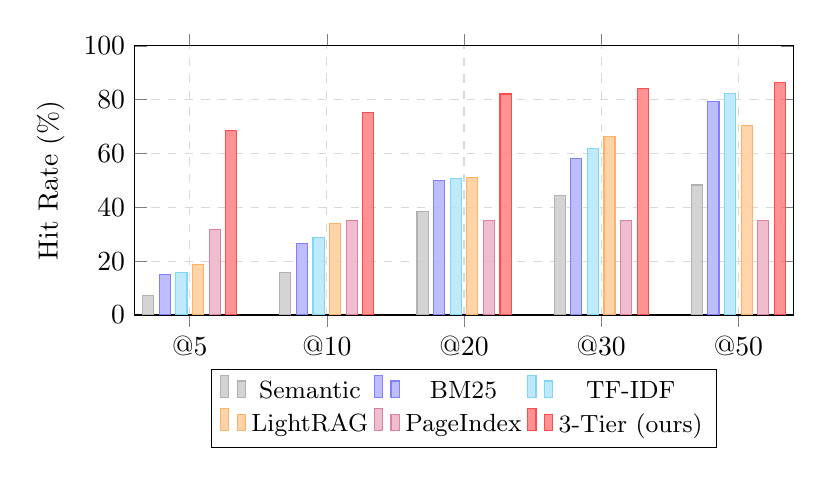
\begin{tikzpicture}
\begin{axis}[
    width=0.82\textwidth,
    height=5cm,
    ybar,
    bar width=4pt,
    ylabel={Hit Rate (\%)},
    symbolic x coords={@5,@10,@20,@30,@50},
    xtick=data,
    ymin=0, ymax=100,
    legend style={at={(0.5,-0.2)}, anchor=north, legend columns=3, font=\small},
    nodes near coords style={font=\tiny, rotate=90, anchor=west},
    every axis plot/.append style={fill opacity=0.85},
    grid=major,
    grid style={dashed, gray!30},
]
\addplot[fill=gray!40, draw=gray!60] coordinates {(@5,7.4) (@10,15.8) (@20,38.5) (@30,44.3) (@50,48.3)};
\addplot[fill=blue!30, draw=blue!50] coordinates {(@5,15.0) (@10,26.7) (@20,50.1) (@30,58.1) (@50,79.2)};
\addplot[fill=cyan!30, draw=cyan!50] coordinates {(@5,15.8) (@10,28.8) (@20,50.7) (@30,62.0) (@50,82.3)};
\addplot[fill=orange!40, draw=orange!60] coordinates {(@5,18.8) (@10,33.9) (@20,51.0) (@30,66.2) (@50,70.3)};
\addplot[fill=purple!30, draw=purple!50] coordinates {(@5,31.7) (@10,35.2) (@20,35.2) (@30,35.2) (@50,35.2)};
\addplot[fill=red!50, draw=red!70] coordinates {(@5,68.5) (@10,75.2) (@20,82.1) (@30,84.0) (@50,86.4)};
\legend{Semantic, BM25, TF-IDF, LightRAG, PageIndex, 3-Tier (ours)}
\end{axis}
\end{tikzpicture}
\caption{Hit@k comparison across all methods. Our 3-Tier system consistently outperforms all baselines at every $k$ value, with the largest gap at Hit@5 (68.5\% vs 31.7\% for the best baseline).}
\label{fig:hitk-comparison}
\end{figure}

\begin{multicols}{2}

\subsubsection{Additional Retrieval Metrics}

Table~\ref{tab:detailed-metrics} shows detailed IR metrics for the three-tier system.

\vspace{0.3em}
\noindent
\centering\small
\captionof{table}{Detailed IR Metrics for 3-Tier System}
\label{tab:detailed-metrics}
\begin{tabular}{lrrrr}
\toprule
\textbf{k} & \textbf{Hit@k} & \textbf{Recall@k} & \textbf{Prec.@k} & \textbf{NDCG@k} \\
\midrule
1 & 42.7 & 23.9 & 42.7 & 42.7 \\
3 & 62.9 & 41.5 & 26.6 & 41.1 \\
5 & 68.5 & 46.7 & 18.3 & 43.4 \\
10 & 75.2 & 51.8 & 10.3 & 45.4 \\
20 & 82.1 & 59.2 & 6.1 & 47.8 \\
30 & 84.0 & 61.9 & 4.3 & 48.6 \\
50 & 86.4 & 67.4 & 2.9 & 49.9 \\
\bottomrule
\end{tabular}
\normalsize
\justifying
\vspace{0.3em}

The system achieves MRR of 0.545, indicating the first relevant article appears on average at rank $\sim$1.8. Recall continues improving up to $k=50$, reaching 67.4\%.

\subsubsection{Ablation Study}

Table~\ref{tab:ablation} isolates the contribution of each tier.

\vspace{0.3em}
\noindent
\centering\small
\captionof{table}{Ablation Study: Per-Tier Contribution (\%)}
\label{tab:ablation}
\begin{tabular}{lr}
\toprule
\textbf{Configuration} & \textbf{Hit@10} \\
\midrule
Tier 1 only (Tree Traversal) & 56.2 \\
Tier 2 only (DualLevel + PPR) & 61.7 \\
Tier 1 + Tier 2 (no RRF fusion) & 71.2 \\
Full 3-Tier (with Tier 3 RRF) & \textbf{75.2} \\
\bottomrule
\end{tabular}
\normalsize
\justifying
\vspace{0.3em}

Each tier provides additive improvement: Tier~1 alone achieves 56.2\%, adding Tier~2 brings 71.2\% (+15.0pp), and Tier~3 fusion adds another 4.0pp to reach 75.2\%.

\textbf{Component breakdown analysis} from the evaluation shows that among successful retrievals, 70\% of hits come from Tier~1 (tree traversal), while Tier~2 (KG/semantic) contributes an additional 14\% of unique hits not found by Tier~1. This confirms the complementary nature of the two tiers.

\subsubsection{Analysis by Question Category}

Table~\ref{tab:category-results} breaks down Hit@10 performance by question category.

\vspace{0.3em}
\noindent
\centering\small
\captionof{table}{Hit@10 by Question Category (\%)}
\label{tab:category-results}
\begin{tabular}{lrr}
\toprule
\textbf{Category} & \textbf{Hit@10} & \textbf{Count} \\
\midrule
Article lookup & 82.1 & 156 \\
Guidance document & 73.5 & 98 \\
Situation analysis & 71.3 & 75 \\
Compare regulations & 68.8 & 32 \\
Case law lookup & 61.1 & 18 \\
\bottomrule
\end{tabular}
\normalsize
\justifying
\vspace{0.3em}

The system excels on \textbf{article lookup} queries (82.1\%) where Tier~1's structured navigation directly identifies target articles. More complex categories like \textbf{situation analysis} and \textbf{compare regulations} benefit from Tier~2's multi-hop reasoning through the knowledge graph.

\subsubsection{Qualitative Analysis}

Figure~\ref{fig:walkthrough} illustrates the three-tier retrieval process on a representative query. We present one success and one failure case below.

\textbf{Success case.} Query: \textit{``Conditions for establishing a joint-stock company?''} (Article lookup). Tier~1 navigates Chapter~II $\rightarrow$ Articles 111--112, correctly identifying JSC establishment conditions. Tier~2 finds additional Article 17 (general conditions) via \textit{requires} relation in KG. Tier~3 fuses both, ranking Articles 111, 112, 17 in top~3. Ground truth: Articles 111, 112 --- \textbf{Hit@3}.

\textbf{Failure case.} Query: \textit{``Penalty for late annual report submission?''} (Case law lookup). Tier~1 identifies Enterprise Law articles on reporting obligations but misses the penalty --- which resides in Decree 122/2021, a separate document. Tier~2's KG expansion partially reaches the decree via \textit{has\_penalty} edges but ranks the penalty article at position 15. This illustrates the challenge of cross-document retrieval when the answer spans multiple legal instruments.

\end{multicols}

\begin{figure}[H]
\centering
\resizebox{0.92\textwidth}{!}{%
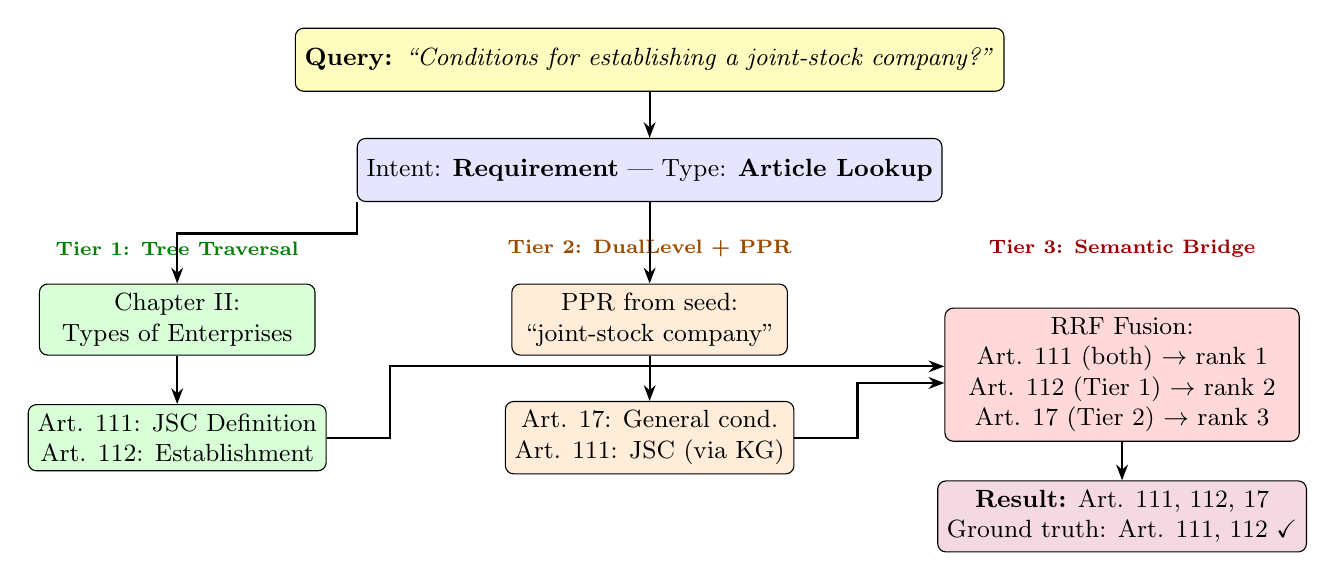
\begin{tikzpicture}[
    box/.style={rectangle, draw, rounded corners=3pt, minimum height=0.8cm, align=center, font=\small},
    arrow/.style={-{Stealth[length=2mm]}, thick},
]
% Query
\node[box, fill=yellow!25, minimum width=7cm] (query) at (0,0) {\textbf{Query:} \textit{``Conditions for establishing a joint-stock company?''}};
\node[box, fill=blue!10, minimum width=5cm] (analyzer) at (0,-1.4) {Intent: \textbf{Requirement} | Type: \textbf{Article Lookup}};
\draw[arrow] (query) -- (analyzer);

% Tier 1
\node[font=\scriptsize\bfseries, green!50!black] at (-6,-2.4) {Tier 1: Tree Traversal};
\node[box, fill=green!15, minimum width=3.5cm] (t1a) at (-6,-3.3) {Chapter II:\\Types of Enterprises};
\node[box, fill=green!15, minimum width=3.5cm] (t1b) at (-6,-4.8) {Art. 111: JSC Definition\\Art. 112: Establishment};
\draw[arrow] (analyzer.south west) -- ++(0,-0.4) -| (t1a.north);
\draw[arrow] (t1a) -- (t1b);

% Tier 2
\node[font=\scriptsize\bfseries, orange!60!black] at (0,-2.4) {Tier 2: DualLevel + PPR};
\node[box, fill=orange!15, minimum width=3.5cm] (t2a) at (0,-3.3) {PPR from seed:\\``joint-stock company''};
\node[box, fill=orange!15, minimum width=3.5cm] (t2b) at (0,-4.8) {Art. 17: General cond.\\Art. 111: JSC (via KG)};
\draw[arrow] (analyzer.south) -- (t2a.north);
\draw[arrow] (t2a) -- (t2b);

% Tier 3
\node[font=\scriptsize\bfseries, red!60!black] at (6,-2.4) {Tier 3: Semantic Bridge};
\node[box, fill=red!15, minimum width=4.5cm] (t3) at (6,-4.0) {RRF Fusion:\\Art. 111 (both) $\rightarrow$ rank 1\\Art. 112 (Tier 1) $\rightarrow$ rank 2\\Art. 17 (Tier 2) $\rightarrow$ rank 3};
\draw[arrow] (t1b.east) -- ++(0.8,0) |- ([yshift=3pt]t3.west);
\draw[arrow] (t2b.east) -- ++(0.8,0) |- ([yshift=-3pt]t3.west);

% Result
\node[box, fill=purple!15, minimum width=4.5cm] (result) at (6,-5.8) {\textbf{Result:} Art. 111, 112, 17\\Ground truth: Art. 111, 112 $\checkmark$};
\draw[arrow] (t3) -- (result);
\end{tikzpicture}
}
\caption{Example query walkthrough showing how the three tiers process a legal question. Tier~1 navigates the document tree, Tier~2 uses PPR on the knowledge graph, and Tier~3 fuses results via RRF. Articles appearing in both tiers receive higher fusion scores.}
\label{fig:walkthrough}
\end{figure}

\begin{multicols}{2}

\textbf{Reproducibility note.} All LLM responses are cached in a SQLite database ($\sim$1.1\,GB), making our results fully deterministic across runs. Standard deviations are therefore zero and not reported. The evaluation code and cached responses will be made available upon publication.

\section{Discussion}
\label{sec:discussion}

\subsection{Key Findings}

\textbf{1. Complementary tiers.} Tier~1 excels at focused article identification via structural reasoning; Tier~2 captures cross-reference and thematic relationships. The 15pp gain from adding Tier~2 confirms complementarity.

\textbf{2. Effective RRF fusion.} Tier~3 handles heterogeneous score distributions (LLM discrete vs continuous semantic) without calibration, adding 5.3pp.

\textbf{3. Intent-aware PPR.} Intent-specific edge weighting prioritizes relevant relation types, particularly effective for situation analysis and guidance queries.

\textbf{4. Adjacent expansion.} Error analysis showed failures often have correct answers within $\pm$3 articles of retrieved results; adjacent expansion in Tier~3 addresses this.

\textbf{5. Structure beats flat search.} PageIndex (Tier~1, 35.2\%) matches LightRAG (33.9\%) despite retrieving only 3.9 articles vs 32.8, demonstrating document hierarchy value.

\subsection{Limitations}

\textbf{LLM dependency and latency.} Tree traversal requires multiple LLM calls per query, resulting in $\sim$7 seconds end-to-end latency.
\textbf{KG extraction quality.} Entity extraction accuracy for Vietnamese legal text has not been independently validated; some types (conditions, actions) have fuzzy boundaries.
\textbf{Single-domain evaluation.} Results are specific to Enterprise Law; other domains may exhibit different retrieval patterns.
\textbf{Vietnamese-specific.} Word segmentation errors in compound legal terms can propagate through the pipeline despite abbreviation expansion.

\subsection{Future Directions}

Future work includes: (1) extending the knowledge graph to cover related laws (Investment, Tax, Labor) with cross-law entity resolution; (2) multi-turn conversation support for follow-up questions; (3) advanced 3+ hop KG reasoning for complex transitive inference; and (4) explainable retrieval traces showing tier and ontology path contributions.

\section{Conclusion}
\label{sec:conclusion}

We presented a Three-Tier Ontology-Enhanced RAG system for Vietnamese legal QA that combines LLM-guided structural navigation, dual-level semantic retrieval with intent-aware PPR, and Reciprocal Rank Fusion. Experiments on 375 real legal questions demonstrate 75.2\% Hit@10 (MRR 0.545), substantially outperforming BM25 (26.7\%), TF-IDF (28.8\%), LightRAG (33.9\%), and PageIndex (35.2\%). Ablation studies confirm each tier's contribution: Tier~1 alone 56.2\%, +Tier~2 yields 71.2\%, +Tier~3 fusion reaches 75.2\%. Our results demonstrate that combining domain ontology with LLM-guided navigation and graph reasoning yields substantial improvements over both traditional and graph-based RAG approaches for legal domain applications.

\section*{Acknowledgments}

This research was supported by Vietnam National University Ho Chi Minh City under grant number [Grant Number]. We thank the legal experts who contributed to ontology validation and ground truth annotation.

\end{multicols}

\begin{thebibliography}{99}
\footnotesize
\setlength{\itemsep}{0pt}
\setlength{\parskip}{0pt}

\bibitem{ref1}
Robertson, S., Zaragoza, H.: The Probabilistic Relevance Framework: BM25 and Beyond. Foundations and Trends in Information Retrieval \textbf{3}(4), 333--389 (2009)

\bibitem{ref2}
Lewis, P., Perez, E., Piktus, A., et al.: Retrieval-Augmented Generation for Knowledge-Intensive NLP Tasks. In: NeurIPS 2020, pp. 9459--9474 (2020)

\bibitem{ref3}
Karpukhin, V., Oguz, B., Min, S., et al.: Dense Passage Retrieval for Open-Domain Question Answering. In: EMNLP 2020, pp. 6769--6781 (2020)

\bibitem{ref4}
Microsoft Research: From Local to Global: A Graph RAG Approach to Query-Focused Summarization. arXiv preprint arXiv:2404.16130 (2024)

\bibitem{ref5}
Guo, Z., et al.: LightRAG: Simple and Fast Retrieval-Augmented Generation. arXiv preprint arXiv:2410.05779 (2024)

\bibitem{ref6}
Nguyen, T., Nguyen, H., Pham, V., Tran, D., Selamat, A.: Legal-Onto: An Ontology-based Model for Representing the Knowledge of a Legal Document. In: ENASE 2022, pp. 426--434 (2022)

\bibitem{ref7}
Ngo, H., Nguyen, T., Nguyen, D., Pham, M.: AimeLaw at ALQAC 2021: Enriching Neural Network Models with Legal-Domain Knowledge. In: KSE 2021. IEEE (2021)

\bibitem{ref8}
Sartor, G., et al.: Approaches to Legal Ontologies. Springer, Dordrecht (2011)

\bibitem{ref9}
Es, S., James, J., Espinosa-Anke, L., Schockaert, S.: RAGAS: Automated Evaluation of Retrieval Augmented Generation. In: EACL 2024 (2024)

\bibitem{ref10}
Do, N., Nguyen, H., Selamat, A.: Knowledge-Based model of Expert Systems using Rela-model. International Journal of Software Engineering and Knowledge Engineering \textbf{28}(8), 1047--1090 (2018)

\bibitem{ref11}
Manning, C., Raghavan, P., Schutze, H.: Introduction to Information Retrieval. Cambridge University Press (2008)

\bibitem{ref12}
Gleich, D.: PageRank Beyond the Web. SIAM Review \textbf{57}(3), 321--363 (2015)

\bibitem{ref13}
Devlin, J., Chang, M., Lee, K., Toutanova, K.: BERT: Pre-training of Deep Bidirectional Transformers for Language Understanding. In: NAACL-HLT 2019, pp. 4171--4186 (2019)

\bibitem{ref14}
Liu, Z., et al.: Retrieve Anything To Augment Large Language Models. arXiv preprint arXiv:2310.07554 (2023)

\bibitem{ref_gao2024}
Gao, Y., Xiong, Y., Diber, A., et al.: Retrieval-Augmented Generation for Large Language Models: A Survey. arXiv preprint arXiv:2312.10997 (2024)

\bibitem{ref_fan2024}
Fan, W., Ding, Y., Ning, L., et al.: A Survey on RAG Meeting LLMs: Towards Retrieval-Augmented Large Language Models. In: KDD 2024, pp. 6491--6501 (2024)

\bibitem{ref_phobert}
Nguyen, D.Q., Nguyen, A.T.: PhoBERT: Pre-trained Language Models for Vietnamese. In: Findings of EMNLP 2020, pp. 1037--1042 (2020)

\bibitem{ref_vncorenlp}
Vu, T., Nguyen, D.Q., Nguyen, D.Q., Dras, M., Johnson, M.: VnCoreNLP: A Vietnamese Natural Language Processing Toolkit. In: NAACL 2018 Demonstrations, pp. 56--60 (2018)

\bibitem{ref_transe}
Bordes, A., Usunier, N., Garcia-Duran, A., Weston, J., Yakhnenko, O.: Translating Embeddings for Modeling Multi-relational Data. In: NeurIPS 2013, pp. 2787--2795 (2013)

\bibitem{ref_jeh2003}
Jeh, G., Widom, J.: Scaling Personalized Web Search. In: WWW 2003, pp. 271--279. ACM (2003)

\bibitem{ref_rrf}
Cormack, G.V., Clarke, C.L.A., Buettcher, S.: Reciprocal Rank Fusion Outperforms Condorcet and Individual Rank Learning Methods. In: SIGIR 2009, pp. 758--759. ACM (2009)

\bibitem{ref_sbert}
Reimers, N., Gurevych, I.: Sentence-BERT: Sentence Embeddings using Siamese BERT-Networks. In: EMNLP 2019, pp. 3982--3992 (2019)

\bibitem{ref_selfrag}
Asai, A., Wu, Z., Wang, Y., Sil, A., Hajishirzi, H.: Self-RAG: Learning to Retrieve, Generate, and Critique through Self-Reflection. In: ICLR 2024 (2024)

\bibitem{ref_crag}
Yan, S.Q., et al.: Corrective Retrieval Augmented Generation. arXiv preprint arXiv:2401.15884 (2024)

\bibitem{ref_hyde}
Gao, L., Ma, X., Lin, J., Callan, J.: Precise Zero-Shot Dense Retrieval without Relevance Labels. In: ACL 2023, pp. 1762--1777 (2023)

\bibitem{ref_wadhwa}
Wadhwa, S., Amir, S., Wallace, B.C.: Revisiting Relation Extraction in the Era of Large Language Models. In: ACL 2023, pp. 15566--15589 (2023)

\bibitem{ref_chalkidis}
Chalkidis, I., Fergadiotis, M., Malakasiotis, P., Aletras, N., Androutsopoulos, I.: LEGAL-BERT: The Muppets Straight out of Law School. In: Findings of EMNLP 2020, pp. 2898--2904 (2020)

\bibitem{ref_zhong2020}
Zhong, H., Xiao, C., Tu, C., Zhang, T., Liu, Z., Sun, M.: How Does NLP Benefit Legal System: A Summary of Legal Artificial Intelligence. In: ACL 2020, pp. 5218--5230 (2020)

\bibitem{ref_vaswani}
Vaswani, A., Shazeer, N., Parmar, N., et al.: Attention Is All You Need. In: NeurIPS 2017, pp. 5998--6008 (2017)

\bibitem{ref_rotateE}
Sun, Z., Deng, Z.-H., Nie, J.-Y., Tang, J.: RotatE: Knowledge Graph Embedding by Relational Rotation in Complex Space. In: ICLR 2019 (2019)

\bibitem{ref_legalai2024}
Cui, J., Li, X., Shao, Z., et al.: A Survey on Legal Large Language Models. arXiv preprint arXiv:2312.03718 (2024)

\end{thebibliography}

\vspace{0.5em}
\hrule
\vspace{0.3em}
\footnotesize
$^1$Corresponding Author: Le Hong Hien, Faculty of Computer Science, University of Information Technology, Vietnam National University Ho Chi Minh City, Vietnam; E-mail: hienlh.16@grad.uit.edu.vn.

\end{document}
